% unicodeは、hyperrefへの指定で、pdfのメタデータにあるタイトルの文字化けを防ぐ
% ptは細かい指定はできないらしい
% チートシート
% https://www.cpt.univ-mrs.fr/~masson/latex/Beamer-appearance-cheat-sheet.pdf
\documentclass[unicode, 14pt, aspectratio=169]{beamer}
% \usepackage{listings}
% \usepackage{enumitem}
% \usepackage{xcolor}
% \usepackage{textcomp}
\usepackage{bussproofs}
\usetheme{titech}
\addbibresource{main.bib}
 \date{\number\year 年\number\month 月\number\day 日}
\title{型理論のはじまり}
\author{\texttt{ryotaro612}}

\newcommand\blfootnote[1]{%
  \begingroup
  \renewcommand\thefootnote{}\footnote{#1}%
  \addtocounter{footnote}{-1}%
  \endgroup
}

\begin{document}
\begin{frame}[noframenumbering, plain]
\titlepage
\end{frame}
\section{導入}
\begin{frame}
  \frametitle{資料の目的}
  {\large 型理論に関わる分野の紹介}
  \par
  \vspace{16pt}
  参考資料に関わる分野
  \begin{itemize}
  \item 論理学
  \item 集合論
  \item 記号論
  \item 構造主義
  \item 哲学、とくに分析哲学
  \end{itemize}
\end{frame}
\section{幾何学}
\begin{frame}
  \frametitle{ギリシアで発展した幾何学}
  {\large 幾何学の知識は\textcolor{highlight}{証明}\footnote{作図を証明とすることもあった。ギリシア語の「証明する」という単語(デイクニュミ)には「図示する」という意味もある。demostrationの語源}された定理の集積}
\begin{columns}
  \begin{column}{0.25\textwidth}
    \begin{center}
      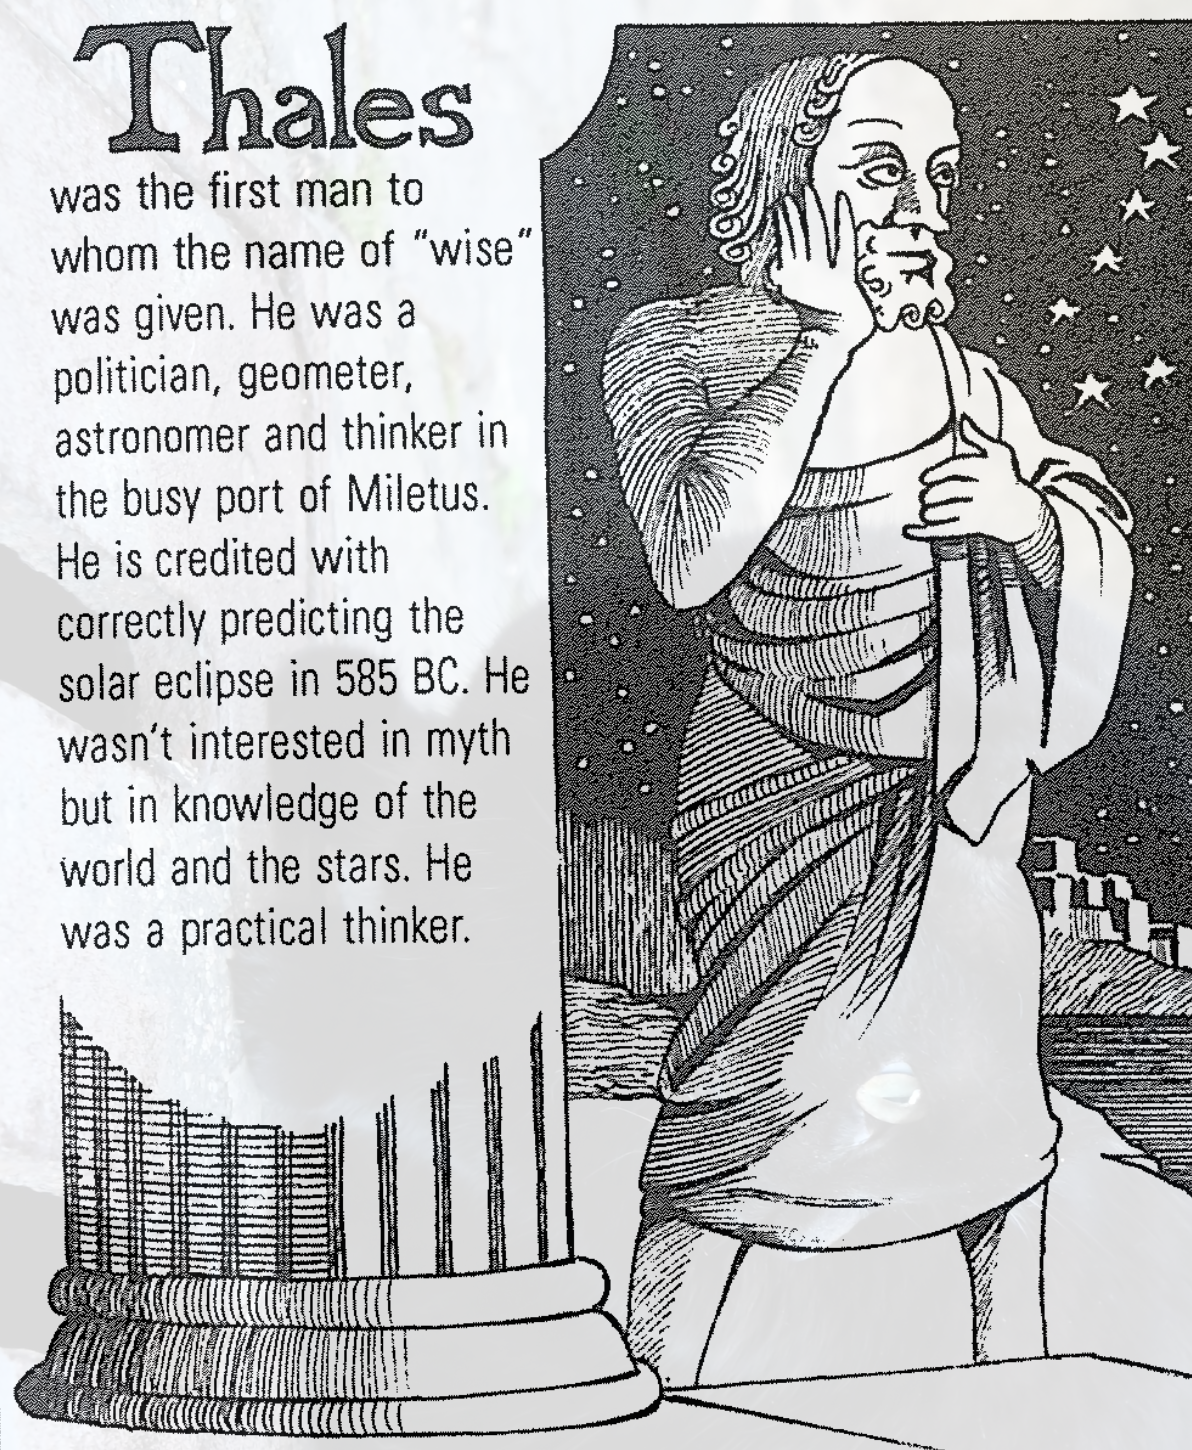
\includegraphics[width=0.7\textwidth]{images/thales.png}
    \end{center}
  \end{column}
  \begin{column}{0.25\textwidth}
    \begin{center}
      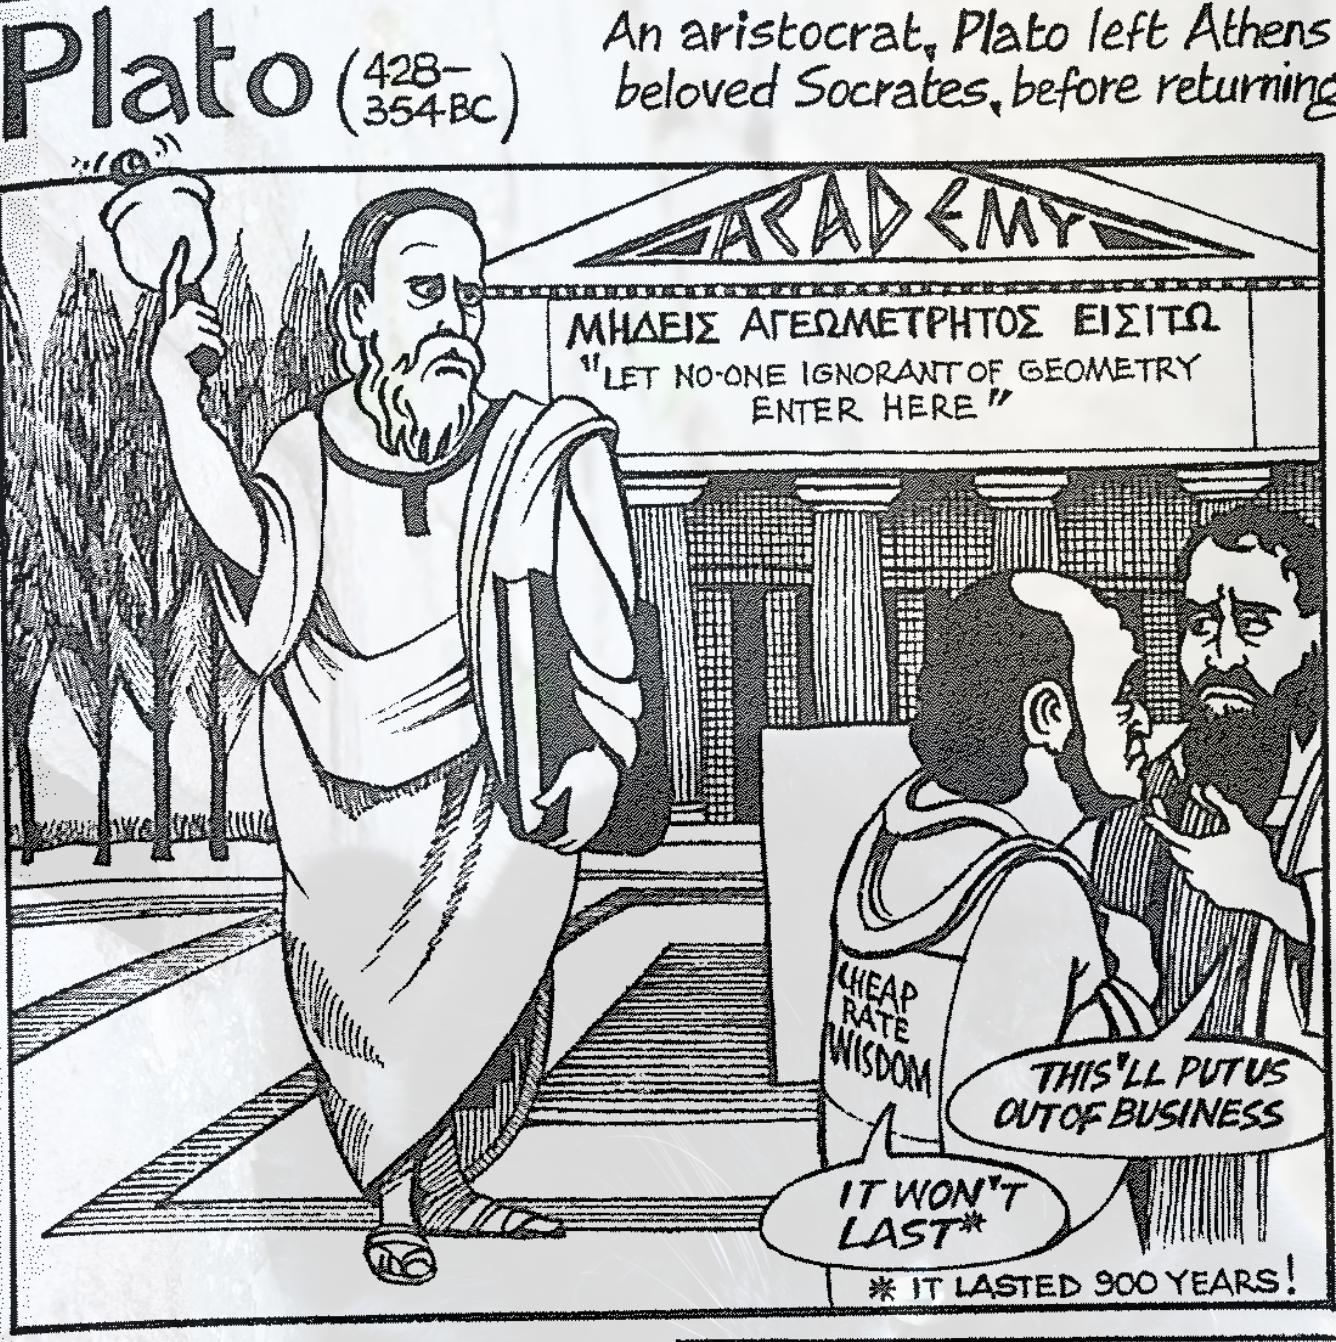
\includegraphics[width=0.7\textwidth]{images/plato.png}
    \end{center}
  \end{column}
  \begin{column}{0.25\textwidth}
    \begin{center}
      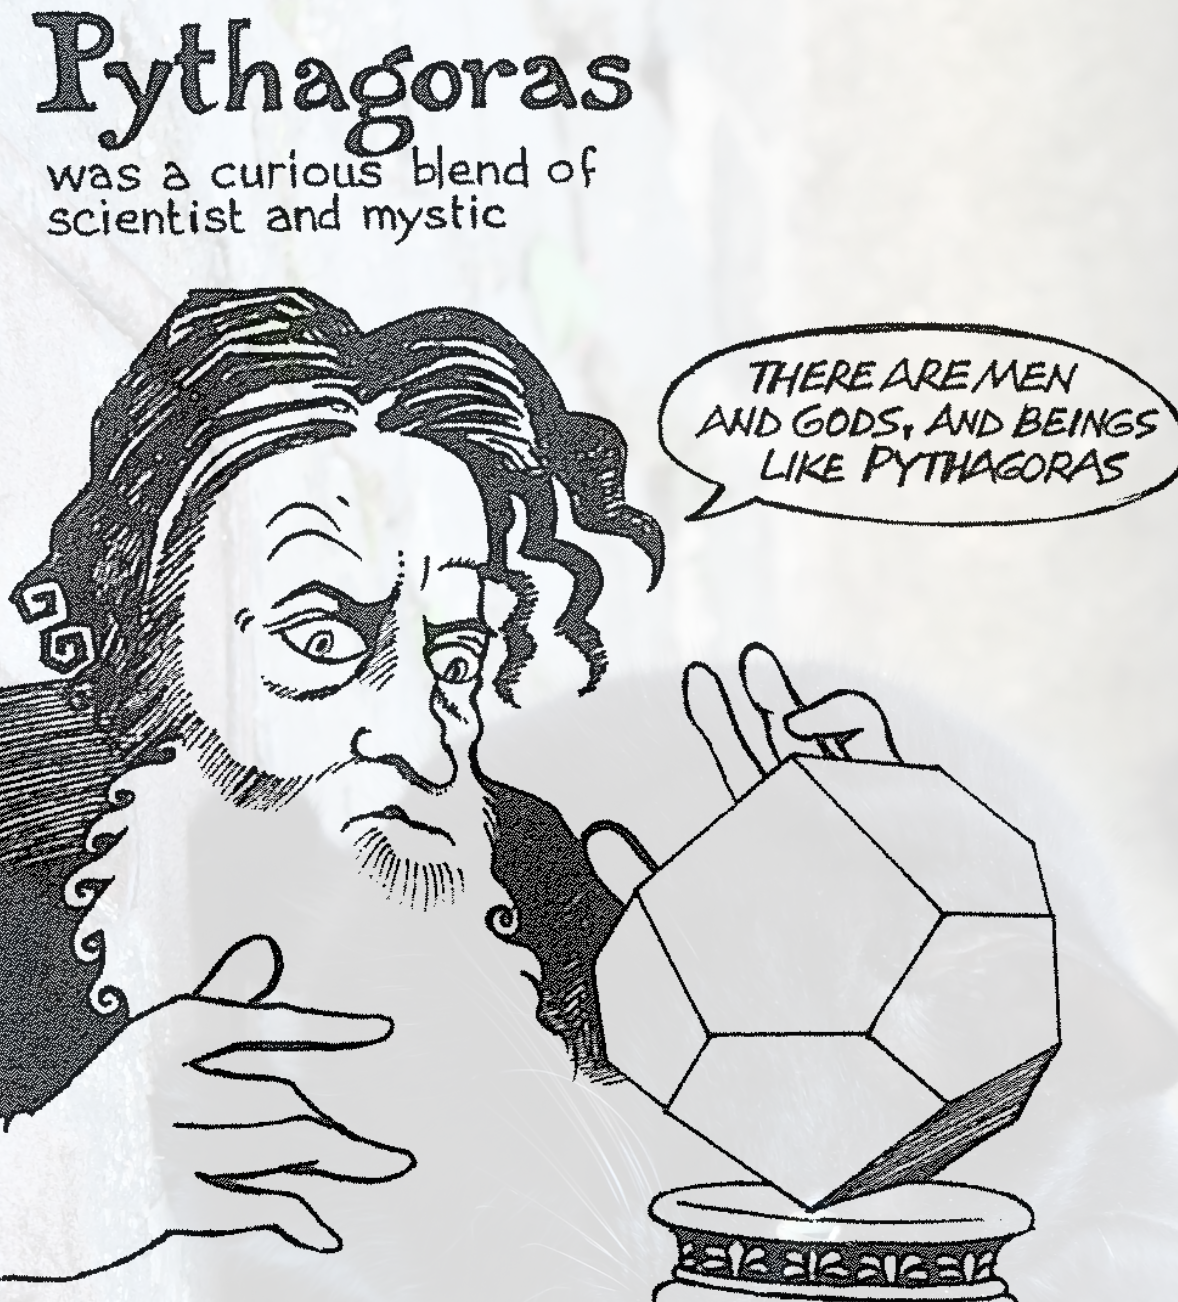
\includegraphics[width=0.7\textwidth]{images/pythagoras.png}
    \end{center}
  \end{column}
  \begin{column}{0.25\textwidth}
    \begin{center}
      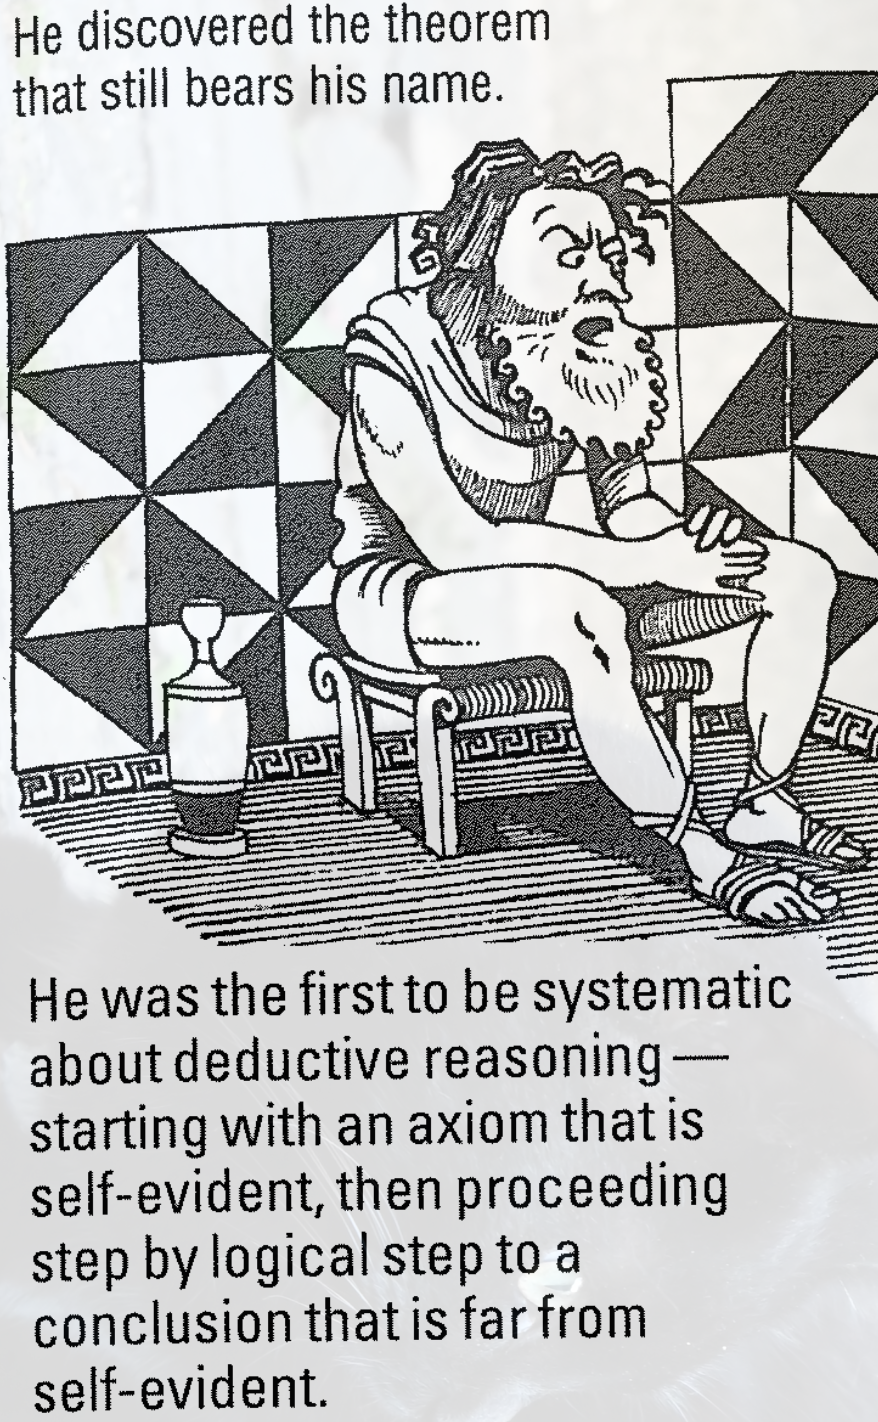
\includegraphics[width=0.7\textwidth]{images/pythagoras2.png}
    \end{center}
  \end{column}  
\end{columns}
\blfootnote{図はPhilosophy for beginners\supercite{philosophy-for-begginers}より} 
\end{frame}
\begin{frame}
  \frametitle{ユークリッドの原論}
  {\large 幾何学が定義、公理、公準\footnote{公理は量などの一般対象の前提、公準は幾何学の対象の前提}、命題、証明に整理された}
  \par
  \vspace{16pt}
  具体例
  \begin{description}
  \item[定義1] 点とは部分をもたないもの
  \item[定義2] 線は幅のない長さ
  \item[定義3] 面は長さと幅だけをもつもの
  \item[公理5] \textcolor{highlight}{全体は部分より大きい}
  \item[命題5] 二等辺三角形の底辺はたがいに等しい
  \end{description}
  
  % ユークリッドはギリシア数学の知識を5つの公準から
\end{frame}
\begin{frame}
  \frametitle{5つの公準}
  {\large 5番目の公準は複雑}
  \par
  \vspace{16pt}  
  \begin{enumerate}
  \item 任意の点から任意の点に直線を引くこと
  \item 有限な線分を連続して直線に延長すること
  \item 任意の点と半径で円を描くこと
  \item すべての直角は等しいこと
  \item \textcolor{highlight}{二直線が一直線と交わるとき、同じ側にできる内角の和が\\二直角よりも小さいなら二直線はその側に延長すると交わる}
  \end{enumerate}
\end{frame}
\begin{frame}[t]
  \frametitle{公準5の別名は平行線公理}
  {\large 公準5を換言すると任意の直線と直線外の任意の一点があるとき一点を通り\textcolor{highlight}{直線に平行な直線は1本}だけ}
  \blfootnote{図は『数学の世界史』\supercite{suugaku-no-sekaishi}より}
  \begin{figure}
    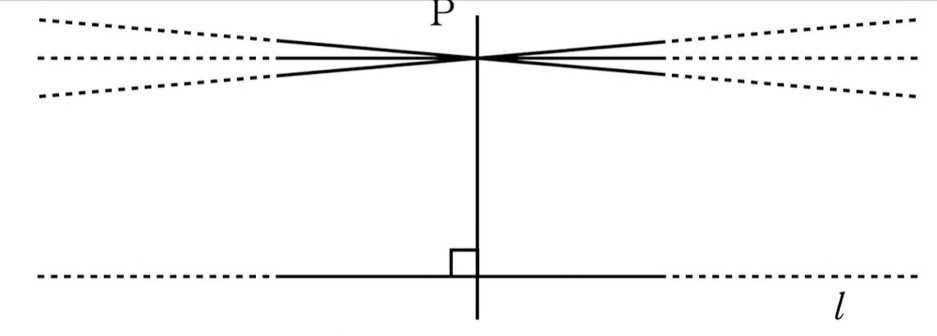
\includegraphics[width=0.7\textwidth]{images/axiom5.png}
    \caption{平行線と平行線にない点$p$を通る直線}
  \end{figure}
\end{frame}
\begin{frame}
  \frametitle{平行線公理への疑問}
  {\large 平行線公理は真理か}
  \begin{itemize}
  \item ほかの公準からの証明できないか
    \begin{itemize}
    \item アラビア世界ではハイタム(965-1039)やハイヤーミー(1048 – 1131)
    \item サッケーリ(1667ー1733), ルシャンドル(1752-1833)は独立に\\
      平行線公理がないと三角形の内角の和は二直角以下になると証明
    \end{itemize}
  \item \textcolor{highlight}{平行線公理を否定しても残りの公準と矛盾しない}
    \begin{itemize}
    \item ガウス(1777-1855)は平行線の公理は証明できないことを示唆する手紙を残す
    \item ロバチェフスキー(1792-1856)とボヤイ(1802-1860)が独立に平行線を二本以上ひけても矛盾しない非ユークリッド幾何学を発見
    \end{itemize}
  \end{itemize}
  % たんなる仮説なのか
  % ほかの公準から導出できるか
% 直線$l$上にない任意の点$P$を通る直線$l$の平行線は2本以上ある
\end{frame}
\begin{frame}
  \frametitle{非ユークリッド空間の例}
  % {\large 測地線があたえられるとき、その測地線にない点pをとおり測地線と交わらない測地線はない}
  {\large 球面の大円は必ず交わる}
  \blfootnote{図は『はじめての構造主義』\supercite{structure}より}
  \begin{figure}
    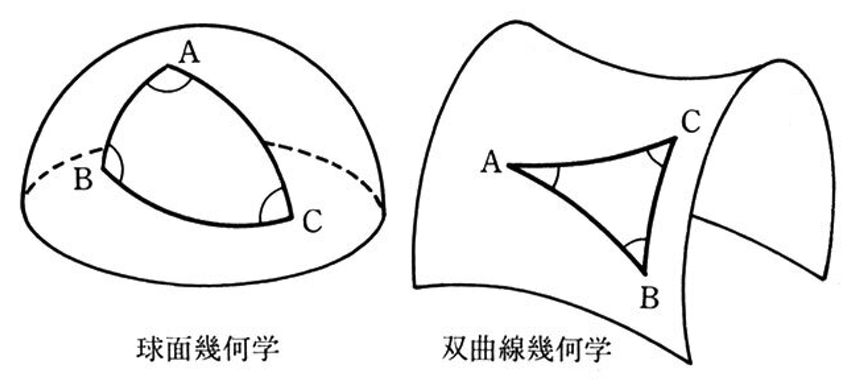
\includegraphics[width=0.5\textwidth]{images/non-euclid.png}
    \caption{非ユークリッド空間の例}
  \end{figure}
  \begin{itemize}
  \item 大円は中心を通る球の切断面
  \item 大円はユークリッド幾何学の直線にあたる
  \end{itemize}
\end{frame}
\section{素朴な集合論}
\begin{frame}
  \frametitle{非ユークリッド幾何学の影響}
  {\large 正しさは仮定した公理から作りだすもの}
  \begin{itemize}
  \item 空間を含む数学の対象は公理から構築するものになる
    \begin{itemize}
    \item ユークリッド幾何学を正しく感じるのは\\素朴な視覚の経験に合うから
    \item 原論の直線や平面の定義はあいまい
    \end{itemize}
  \item 数学の対象を定義する道具としてデデキントとカントールは\textcolor{highlight}{集合論}を確立
  \end{itemize}
\end{frame}
\begin{frame}
  \frametitle{ものの集まりで数学を考える}
  {\large 空集合だけで対象を定義できる}
  \par
  例
  \begin{enumerate}
  \item 空集合$\phi$を$\{x|x\neq x\}$とする
  \item $\phi$を$0$となづける
  \item 空集合1つからなる集合$\{\phi\}$を$1$となづける
  \item $\{0, 1\}$を$2$となづける
  \item $\vdots$
  \item $\{0, 1, 2, \cdots\}$を$\omega$となづける
  \item $\omega$の積集合$P(\omega)$を実数全体の集合にする
  \item $P(P(\omega))$を実数から実数への関数の集合にする
  \end{enumerate}
\end{frame}
\section{記号論理学}
\begin{frame}
  \frametitle{算術の基礎}
  {\large フレーゲは論理学を算術の基礎におこうとした}
  \begin{columns}
    \begin{column}{0.8\textwidth}
      \begin{itemize}
      \item 「概念記法(Begriffsschrift)」で述語論理を提案
      \item 「算術の基本法則」で概念記法と集合論による算術の公理と定理を提案
      \item 語にはsenseとreferenceがあると提起
        \begin{itemize}
        \item 明けの明星と宵の明星のreferenceは金星
        \item 「金星は明けの明星である」と「金星は金星である」のsenseは違う
        \end{itemize}
      \end{itemize}
    \end{column}    
    \begin{column}{0.2\textwidth}
      \begin{figure}
        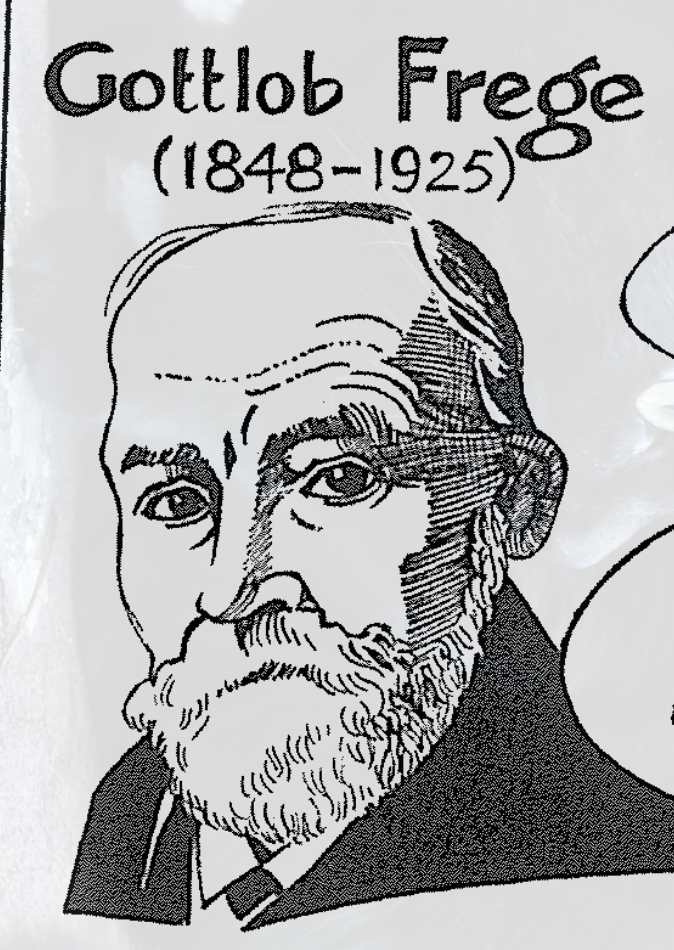
\includegraphics[width=1\textwidth]{images/frege.png}
      \end{figure}       
    \end{column} 
  \end{columns}
  \blfootnote{図はPhilosophy for beginners\supercite{philosophy-for-begginers}より}
\end{frame}
\begin{frame}
  \frametitle{思考を記号で計算する}
  {\large 推論を記号操作に還元する考えは17世紀以前からある}  
  \begin{columns}
    \begin{column}{0.55\textwidth}
      考案したもの
      \begin{itemize}
        \item 今日で使う微積分学の記法
        \item 二進数
        \item characteristica universalis
          \begin{itemize}
          \item 単語を構成するアルファベットのような思考の記号体系
          \item 代数的な記号操作で推論
          \end{itemize}
      \end{itemize}
    \end{column}    
    \begin{column}{0.4\textwidth}
      \begin{figure}
        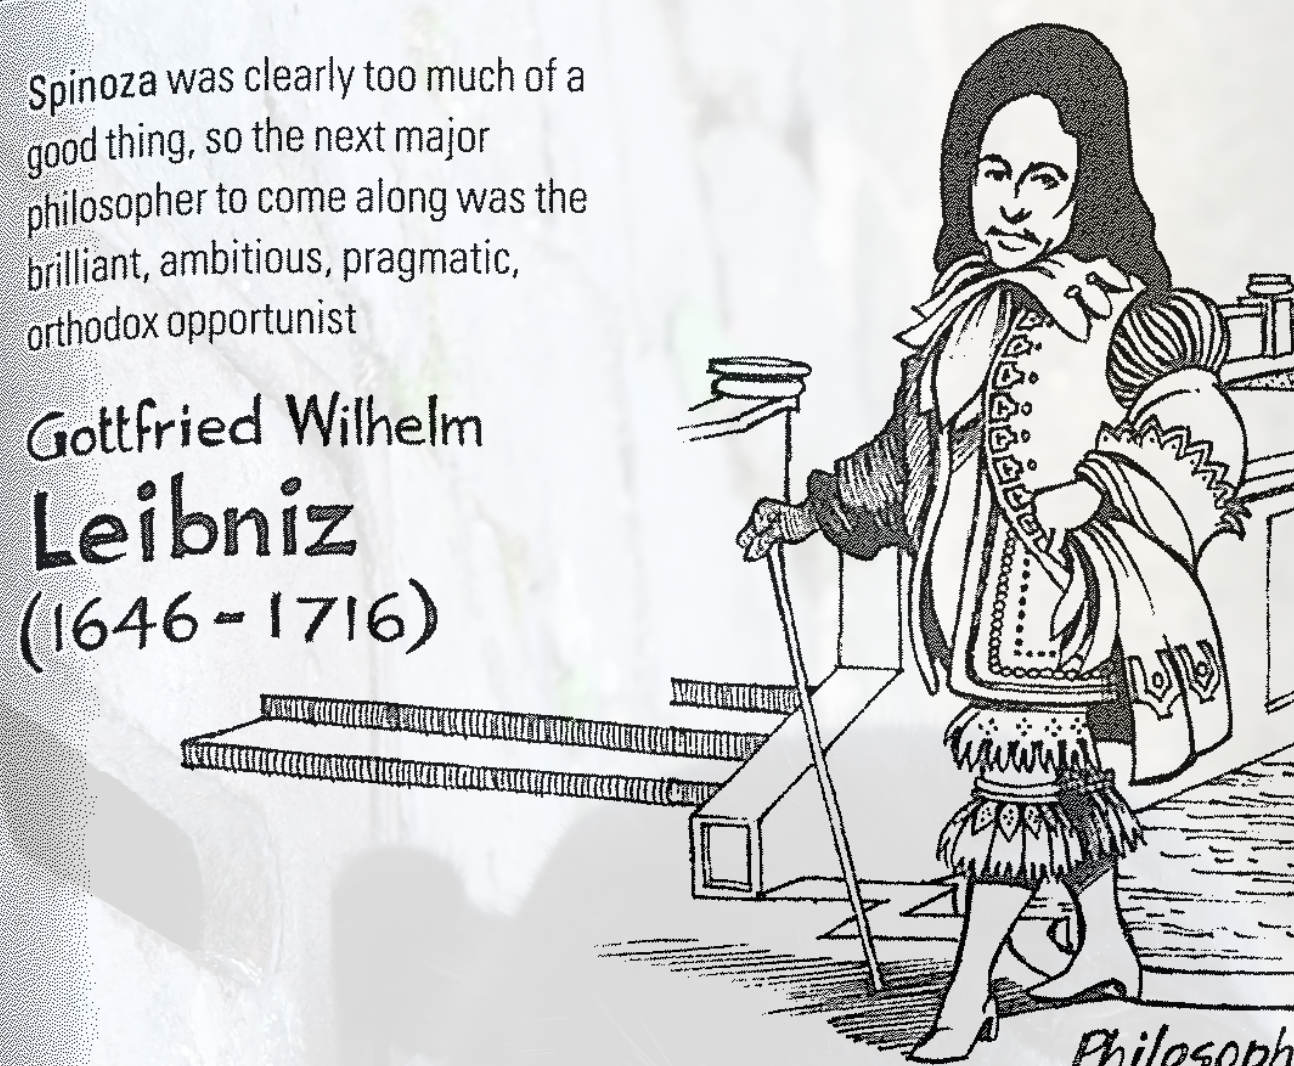
\includegraphics[width=0.7\linewidth]{images/leibniz.png}
        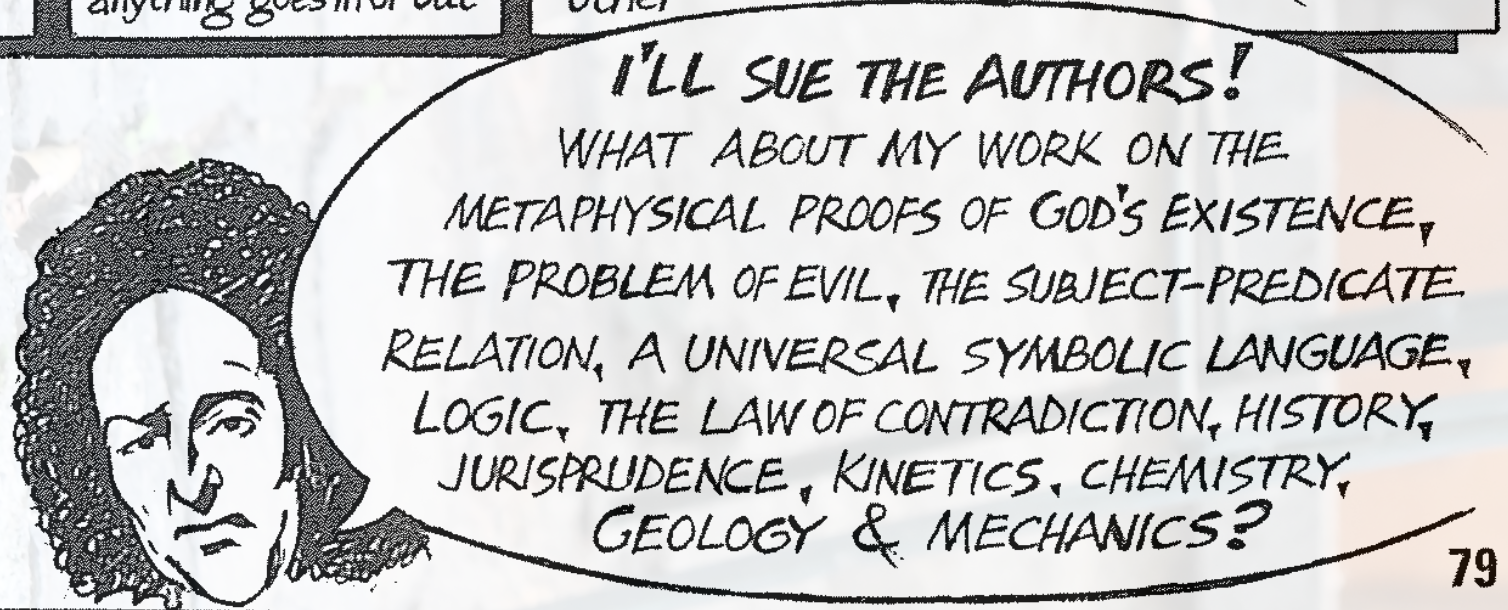
\includegraphics[width=0.7\linewidth]{images/universal.png}
      \end{figure}       
    \end{column} 
  \end{columns}
  \blfootnote{図はPhilosophy for beginners\supercite{philosophy-for-begginers}より}  
\end{frame}
\begin{frame}
  \frametitle{ブールの論理代数}
  {\large ブールは命題に出現する個体の集合を記号で表した}
  \begin{columns}
    \begin{column}{0.7\textwidth}
      \begin{center}
        THE LAWS OF THOUGHT\supercite{bool}より引用
        \begin{quotation}
          Let us then agree to represent the class of individuals to which a particular name or description is applicable, by a single letter, as x. If the name is “men,” for instance, let x represent “all men,”
        \end{quotation}
      \end{center}
    \end{column}    
    \begin{column}{0.2\textwidth}
      \begin{figure}
        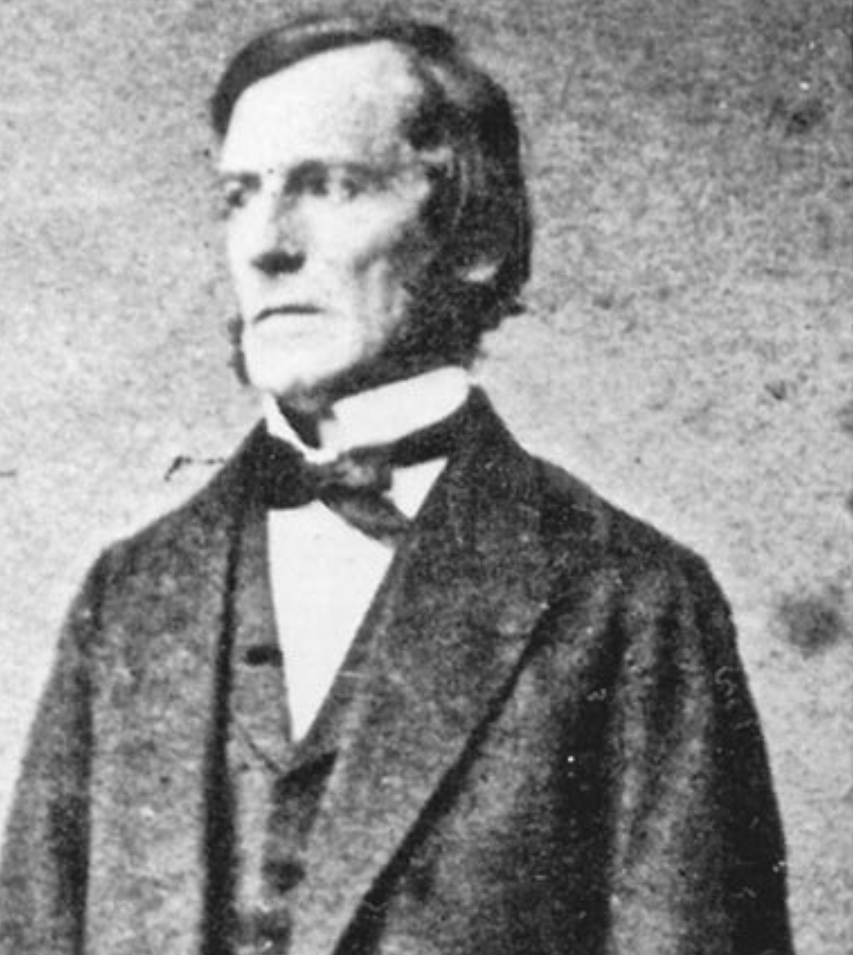
\includegraphics[width=1\textwidth]{images/bool.png}
      \end{figure}       
    \end{column} 
  \end{columns}
  \blfootnote{図は``The Universal Computer: The Road from Leibniz to Turing''より}
\end{frame}
\begin{frame}
  \frametitle{推論規則の例}
  {\large 命題論理は、命題と論理結合子からなる論理体系}
  \par
  推論規則
  \par
  \vspace{16pt}
  \AxiomC{$\varphi, \psi$}
  \RightLabel{(\wedge 導入)}
  \UnaryInfC{$\varphi\wedge\psi$}
  \DisplayProof
  \AxiomC{$\varphi\wedge\psi$}
  \RightLabel{(\vee 消去)}
  \UnaryInfC{$\varphi$}
  \DisplayProof
  \AxiomC{$\varphi\wedge\psi$}
  \RightLabel{(\vee 消去)}
  \UnaryInfC{$\psi$}
  \DisplayProof
  \AxiomC{$[\varphi]$}
  \noLine
  \UnaryInfC{$\vdots$}
  \noLine
  \UnaryInfC{$\psi$}
  \RightLabel{(\rightarrow 導入)}  
  \UnaryInfC{$\varphi\rightarrow\psi$}
  \DisplayProof
  \AxiomC{$\varphi$}
  \AxiomC{$\varphi\rightarrow\psi$}
  \RightLabel{(\rightarrow 消去)}  
  \BinaryInfC{$\psi$}
  \DisplayProof
  \AxiomC{$\bot$}
  \RightLabel{($\bot$)}
  \UnaryInfC{$\varphi$}
  \DisplayProof
  \AxiomC{$[\neg\varphi]$}
  \noLine
  \UnaryInfC{$\vdots$}
  \noLine
  \UnaryInfC{$\bot$}
  \RightLabel{(背理法)}
  \UnaryInfC{$\varphi$}
  \DisplayProof  
\end{frame}
\begin{frame}
  \frametitle{概念記法}
  {\large フレーゲは述語の言明を形式化した}
  \begin{itemize}
  \item 「$\varphi$が〜である」言明を、引数$\varphi$を真偽値に写像する述語$P(\varphi)$を命題論理に加える
  \item 「任意の$\phi$について」という普遍量化子$\forall$と、「ある$x$について」という存在量化子$\exists$も加える
  \item たとえば「家にいるペットは犬か猫だ」という命題は$\forall x. P(x) \rightarrow D(x)\vee C(x)$のように表せる
  \item 複雑な命題を単純な命題の組合せで表現しやすくなる
  \end{itemize}
  % \AxiomC{$A[t]$}
  % \RightLabel{(\forall 導入)}
  % \UnaryInfC{$\forall x A[x]$}
  % \DisplayProof
  % \AxiomC{$\forall x A[x]$}
  % \RightLabel{(\forall 消去)}
  % \UnaryInfC{$A[t]$}
  % \DisplayProof
  % \AxiomC{$A[t]$}
  % \RightLabel{(\exists 消去)}
  % \UnaryInfC{$\exists A[x]$}
  % \DisplayProof
  
\end{frame}
\begin{frame}
  \frametitle{ラッセルのパラドクス}
  {\large 集合の集合を考えると矛盾がおきる}
  \begin{itemize}
  \item ラッセルのパラドクス
    \begin{enumerate}
    \item 自分自身を元にもたない集合すべての集合を$R=\{x|x\notin x \}$とする
    \item $R$が自分を元にもたない集合とすると、定義から$R$は$R$の元になる
    \item $R$が自分を元にもつ集合とすると、定義から$R$は$R$の元ではない
    \end{enumerate}
  \item 算術の基本法則では、第五公理$\epsilon P=\epsilon Q \equiv \forall x [P(x)\equiv Q(x)]$がパラドクスを招く
    \begin{itemize}
    \item 公理は述語の同一である条件
    \item $\epsilon P$は述語$P$を充足する集合
    \end{itemize}
      \begin{enumerate}
    \item $R$を述語論理で$\exists P[x=\epsilon P\wedge \neg P(x)]$と表せる
    \item $x$を$\epsilon R$とすると$R(\epsilon R)\equiv\neg R(\epsilon R)$となる
    \end{enumerate}
  \item ラッセルが述語論理の述語は述語をとれない規則のような階層構造でパラドクスの解消を試みたのが型理論のはじまり
  \end{itemize}
\end{frame}
\begin{frame}
  \frametitle{型の概念}
  ラッセルの自分自身に言明する述語の例に対して、フレーゲは述語は述語を引数にとれないと回答した
  ただし述語の外延が作用する
\end{frame}
% https://fair-use.org/bertrand-russell/the-principles-of-mathematics/s498
% https://plato.stanford.edu/entries/type-theory/
% https://people.umass.edu/klement/pom/pom-portrait.pdf
% https://repository.kulib.kyoto-u.ac.jp/dspace/bitstream/2433/151121/1/ronso38_S49_type.pdf
% https://www.britannica.com/topic/theory-of-types-logic
\begin{frame}[allowframebreaks,t]
  \frametitle{参考資料}
  \printbibliography
  \nocite{*}
\end{frame}

\end{document}
